\documentclass{article}
\usepackage{graphicx} 

\title{A Dinâmica Social dos "Parças": Uma Análise sobre a Amizade}
\author{Gemini}
\date{Abril 2026}

\renewcommand{\contentsname}{Sumário}

\renewcommand{\listtablename}{Lista de Tabelas}

\renewcommand{\listfigurename}{Lista de Figuras}

\begin{document}

\maketitle

\tableofcontents

\listoftables

\listoffigures

\section{Introdução}
A amizade é um fenômeno sociocognitivo que transcende barreiras geográficas e culturais. Diferente de laços sanguíneos, a amizade baseia-se na escolha deliberada e na manutenção de algoritmos de confiança mútua. Este artigo explora como pequenos gestos e a convivência frequente solidificam esses vínculos.

\section{Elementos Fundamentais de um Vínculo}

\subsection{O Pilar da Reciprocidade}
Para que uma amizade seja classificada como "verdadeira", alguns componentes são indispensáveis. De acordo com a literatura popular, podemos listar:

\begin{enumerate}
\item \textbf{Lealdade}: Estar \underline{presente} mesmo quando não há \textit{Wi-Fi} disponível.

\item \textbf{Humor Compartilhado}: Entender piadas que ninguém mais entende.
\end{enumerate}


\subsection{A Gestão de Conflitos}
Amizades sólidas não são ausentes de brigas, mas sim eficientes na resolução de disputas sobre qual filme assistir no cinema.

\section{A Matemática da Proximidade}
Podemos modelar o Nível de Amizade ($A$) através de uma equação simples, onde consideramos o tempo de convivência ($t$) e a quantidade de memes trocados ($m$):
\begin{equation}
A = \int_{0}^{t} \frac{m \cdot \cos(\theta)}{d^2} \, dt
\end{equation}


\section{Categorização de Interações Sociais}

\subsection{Eventos de Baixo Impacto}
Nesta categoria, enquadram-se cafés rápidos e conversas por áudio de 10 minutos que poderiam ter sido um texto.

\subsection{Eventos de Alto Risco (The "Chaos" Tier)}
Aqui o nível de estresse e diversão aumenta proporcionalmente. A tabela abaixo resume as métricas dessas interações:
\begin{table}[h]
\centering
\begin{tabular}{lll}
\hline
\textbf{Atividade} & \textbf{Nível de Caos} & \textbf{Gasto Médio} \\
\hline
Noite de Jogos & Crítico & R\$ 50,00 \\
\hline
Viagem de Carro & Imprevisível & Elevado \\
\hline
Karaokê em Grupo & Auditivo & Moderado \\
\hline
\end{tabular}
\caption{Métricas de interações sociais de alto risco}
\label{tab:caos}
\end{table}


\section{Representação Visual do Suporte Emocional}
\begin{figure}[h]
\centering
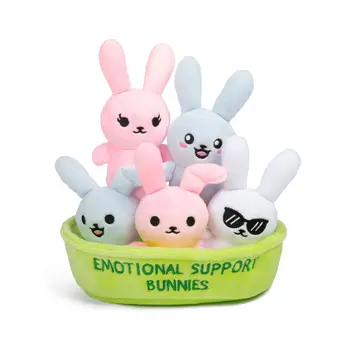
\includegraphics[scale=0.2]{img/suporte.png}
\caption{Suporte emocional.}
\label{fig:suporte}
\end{figure}


\section{Conclusão}
Em suma, a amizade não é apenas um conceito abstrato. Como afirmado em estudos clássicos, a vida é curta demais para não ter alguém para dividir a batata frita.
Segundo \cite{souza2013amizade} a amizade contribui para o bem-estar subjetivo.

\bibliographystyle{plain} 
\bibliography{referencias.bib}

\end{document}
